\section{Circuito N° 3: Rectificador de precisión }

\subsection{Análisis Teórico}

\begin{figure}[H]
    \centering
    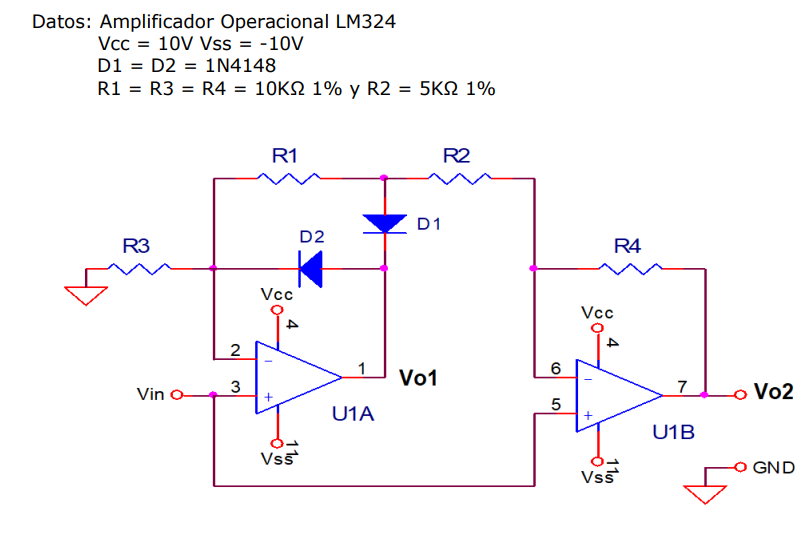
\includegraphics[width=0.5\linewidth]{Secciones/Circuito3/circuito.png}
    \caption{Circuito del rectificador}
    \label{fig:Circuito3}
\end{figure}

Para determinar la tensión de salida Vo en función de la tensión de entrada Vin, se considerarán dos casos: cuando la tensión de entrada es positiva, y cuando la tensión de entrada es negativa.

\[V_0 = f(V_{in}) \ \text{con} \ 0 < V_{in}\]

En estas condiciones, el diodo D2 conduce, mientras que el diodo D1 no, ya que el amplificador U1A se encuentra operando en modo no inversor.
Inicialmente se analizará el caso en que la tensión de entrada del amplificador U1B se encuentra pasivada, entonces la ecuación de corrientes en el nodo ‘6’ resulta:

\begin{equation}
\frac{V_o}{R_4} = \frac{V_in}{R_1 + R_2}
\end{equation}

\begin{equation}
\frac{V_o}{10[k\Omega]} = -\frac{V_{in}}{15[k\Omega]}
\end{equation}

\begin{equation}
V_o = - \frac{2}{3}V_{in}
\end{equation}

Si ahora se pasiva la tensión de entrada del amplificador U1A, se plantea el divisor de tensión en el nodo ‘6’:

\[V_{in} = V_o \frac{R_1+R_2}{R_1+R_2+R_4}\]

\[V_{in} = V_o \frac{15[k\Omega]}{25[k\Omega]}\]

\[V_o = \frac{5}{3}V_{in}\]

Si no se tiene ninguna tensión pasivada, aplicando superposición:

\[V_o = \frac{5}{3}V_{in} - \frac{2}{3}V_{in}\]

\[V_o = V_{in}\]


\subsection{Vo = Vin con 0 \texorpdfstring{$>$}{>} Vin}


En estas nuevas condiciones, el diodo D1 conduce, mientras que el diodo D2 no. Se considerará inicialmente que la tensión a la salida del amplificador U1A se encuentra pasivada. Se plantea el divisor de tensión en el nodo ‘6’:

\[V_{in} = V_o \frac{R_2}{R_2+R_4}\]

\[V_{in} = V_o \frac{5 k\Omega}{15 k\Omega }\]

\[V_o = 3V_{in}\]

Si ahora se considera que la tensión de entrada del amplificador U1B está pasivada, la ecuación de corrientes del nodo ‘6’, tomando VoB como la tensión de salida del amplificador U1B, resulta:

\begin{equation}
\frac{V_{oB}}{R_2} = - \frac{V_o}{R_4}
\end{equation}

\begin{equation}
\frac{V_{oB}}{5 [k\Omega]} = - \frac{V_o}{10 [k\Omega]}
\end{equation}

\begin{equation}
V_o = - 2V_{oB}
\end{equation}

Por otro lado, la tensión de salida VoB se obtiene planteando el divisor de tensión del amplificador U1B:

\[V_{in} = V_{oB} \frac{R_3}{R_1+R_3}\]

\[V_{in} = V_{oB} \frac{10 [k\Omega]}{20 [k\Omega]}\]

\[V_{in} = \frac{1}{2}V_{oB}\]

Reemplazando:

\[V_o = - 4V{in}\]

Si no se tiene ninguna tensión pasivada, aplicando superposición:

\[V_o = 3V{in} - 4V{in}\]

\[V_o = - V{in} \]

En resumen, cuando la tensión de entrada es positiva, la tensión de salida es igual a la tensión de entrada, mientras que cuando la tensión de entrada es negativa, la tensión de salida será positiva y de igual amplitud a la de entrada.


\subsection{Simulación}
Después de encontrar analíticamente la expresión de la tensión de salida en función de aquella de entrada, se simuló el circuito con el software LTSpice. En la figura \ref{fig:TP1_3_Vo1_Vo2_Vin_vs_t}, se visualiza la tensión de salida para una entrada senoidal. 

\begin{figure}[H]
    \centering
    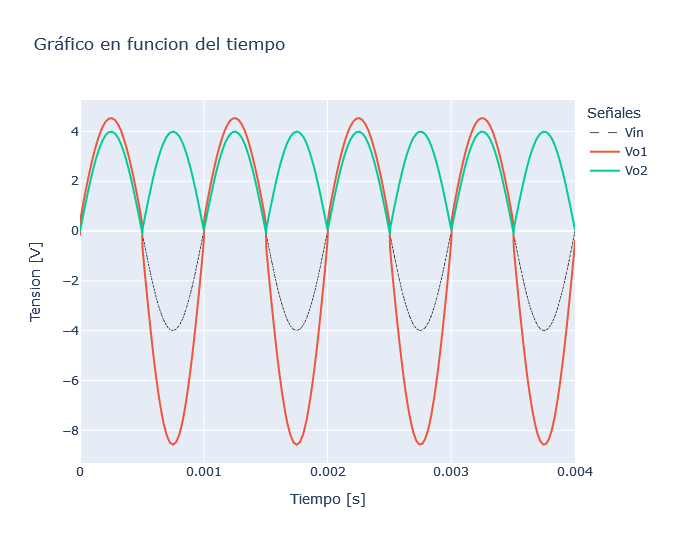
\includegraphics[width=0.9\linewidth]{Secciones/Circuito3/TP1_3_Vo1_Vo2_Vin_vs_t.png}
    \caption{Tensiones de salida del rectificador}
    \label{fig:TP1_3_Vo1_Vo2_Vin_vs_t}
\end{figure}

Para terminar, se graficó la evolución de la amplitud de la señal de salida en función de aquella de la señal de entrada y se observó que la amplitud maxima para una entrada senoidal es de 4 V.

\begin{figure}[H]
    \centering
    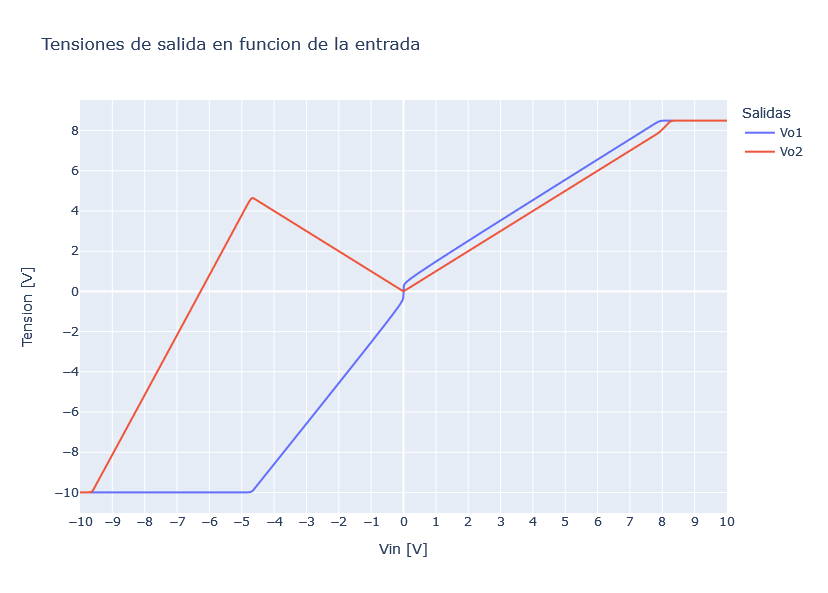
\includegraphics[width=0.9\linewidth]{Secciones/Circuito3/TP1_3_Vo1_Vo2_vs_Vin.png}
    \caption{Simulación entrada/salida del rectificador}
    \label{fig:TP1_3_Vo1_Vo2_vs_Vin}
\end{figure}

\begin{table}[H]
\centering
\begin{tabular}{|c|c|c|c|}
\hline
\textbf{Vin [V]} & \textbf{Vout 1 [V]} & \textbf{Vout 2 [V]} \\ \hline
 10 m &  280 m &   9,75 m \\ \hline
 50 m &  394 m &  49,7  m \\ \hline
100 m &  475 m &  99,8  m \\ \hline
500 m &  948 m & 499    m \\ \hline
    1 & 1,48   &   1      \\ \hline
    2 & 2,51   &   2      \\ \hline
\end{tabular}
\caption{Tensiones de salida según Vin.}
\label{tab:TP1_3_Vo1_Vo2_vs_Vin}
\end{table}

\subsection{Implementación}
A partir del PCB realizado se midió la salida de los dos operacionales en el rectificador.

\begin{figure}[H]
    \centering
    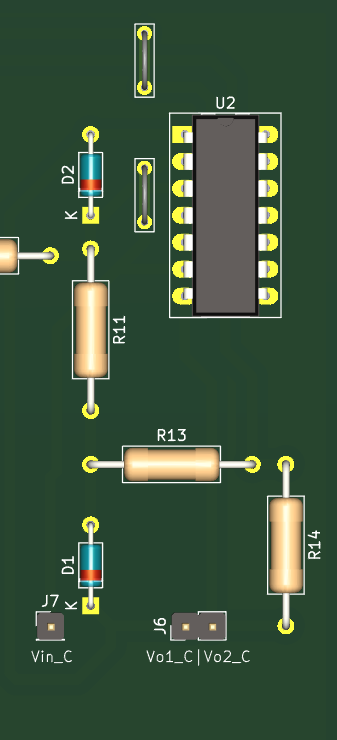
\includegraphics[width=0.5\linewidth]{Secciones//Circuito3/pcb3.png}
    \caption{Salidas del rectificador $Vo1_C$ y $Vo2_C$, y su entrada $Vin_C$ en el PCB}
    \label{fig:enter-label}
\end{figure}

Cuando se armo el circuito, se colocó una resistencia de 4,7K en el lugar de R2 por la falta de disponibilidad de resistencias de 5K. Esto causó que los ciclos rectificados no sean iguales en amplitud, debido a que $V_o \neq V_{in}$ numéricamente.

\begin{figure}[H]
    \centering
    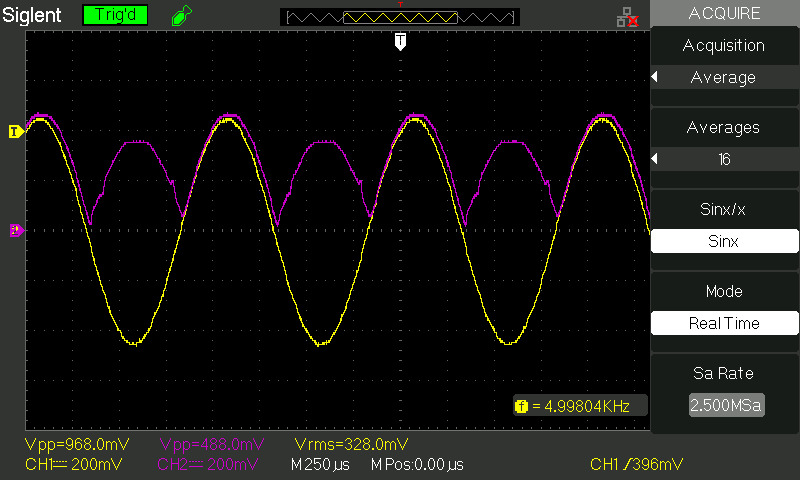
\includegraphics[width=0.75\linewidth]{Secciones//Circuito4/osc4_1.jpg}
    \caption{En violeta $Vo_2$ y en amarillo $V_{in}$. Notar la diferencia de amplitud entre dos picos consecutivos.}
    \label{fig:enter-label}
\end{figure}

Al reajustar R2 usando un preset, se logró alcanzar la simetría obtenida mediante la simulación.

\begin{figure}[H]
    \centering
    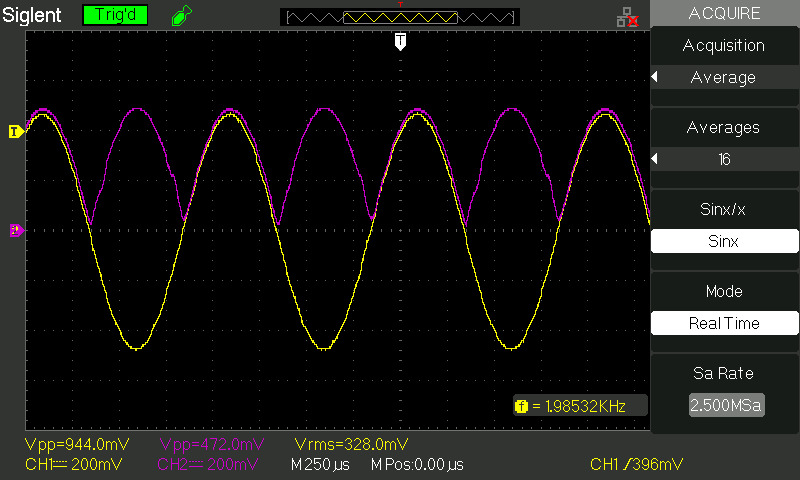
\includegraphics[width=0.75\linewidth]{Secciones//Circuito3/osc3_2.jpg}
    \caption{La amplitud se vuelve uniforme al corregir la resistencia}
    \label{fig:enter-label}
\end{figure}

Al la salida $Vo1$, se observa una senoidal distorsionada. Esto es causado por las alinealidades del circuito, corregidas en el posterior operacional.

\begin{figure}[H]
    \centering
    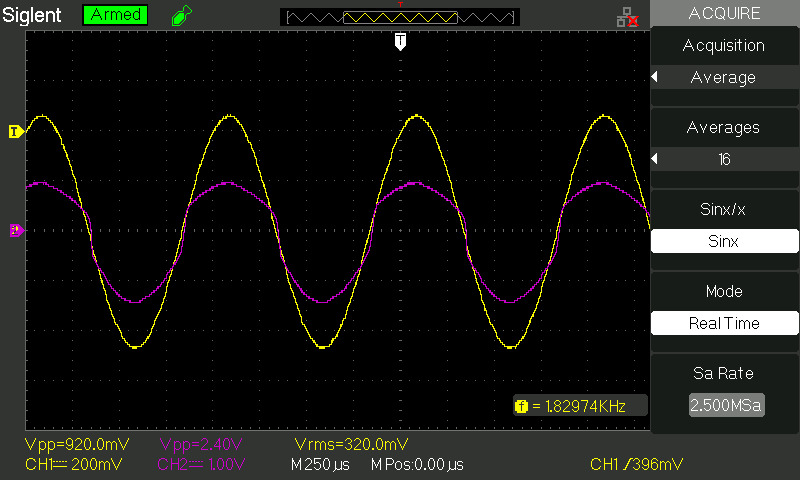
\includegraphics[width=0.75\linewidth]{Secciones//Circuito3/osc3_3.jpg}
    \caption{En violeta $Vo_1$ y en amarillo $V_{in}$.}
    \label{fig:enter-label}
\end{figure}
%\subsection{Experimental}

%En el análisis de modo común:




%\subsection{II.4. Comparación de los resultados teóricos, de simulación y experimentales}

%En la siguiente tabla, reunimos los resultados obtenidos por teoricamente, por simulación y experimentalmente. También calculamos los errores relativos entre los resultados obtenidos experimentalmente con los resultados obtenidos por simulación y teóricamente.
%Para Vin=1V y Vin=3V, los errores relativos entre simulación y teoría son extremadamente pequeños (menor a 1%), como previamente. Para esos valores de Vin, los errores exp/simu y exp/teoría quedan bastante pequeños (con un máximo de 10,4%).
%En contrario, podemos ver que para valores más altos de Vin, los errores son mucho más grandes porque ocurre el fenómeno de saturación o sea que la tensión de salida es físicamente limitada por la tensión de alimentación del operador operacional. El gráfico de la Figura 35 permite una mejor visualización de esas conclusiones.


